\documentclass[11pt]{article}
\usepackage{acl2014}
\usepackage{times}
\usepackage{url}
\usepackage{latexsym}


%pseudocode:
\usepackage{algorithm}
\usepackage{algpseudocode} 

%figures:
\usepackage{tikz}
\usetikzlibrary{trees,positioning,backgrounds}
\usepackage{tikz-qtree}

%references and keeping floats in place
\usepackage{hyperref}
\usepackage[section]{placeins}

\usepackage{amsmath} 

\title{Doubling \dops \\ 
{\normalsize A comparison of \ddop~and \dops}}
\author{Benno Kruit\\10576223\\\And
Sara Veldhoen\\10545298\\}
\date{}


\begin{document}
%NB: gebruik \dops{} of \dops~ om netjes een whitespace erachter te krijgen in lopende tekst
\newcommand{\dops}[0]{DOP$ ^*$}
\newcommand{\ddop}[0]{Double-DOP}

\maketitle

\begin{abstract}
This paper investigates two models of the Data Oriented Parsing approach to natural language syntax. We assess the theoretical and practical differences between these models by comparing the grammars they derive.
\end{abstract}


\section{Introduction}
%Introduction to the paper
%General introduction to the DOP framework, terminology 
%NB: introduce term 'fragment' for usage throughout this document



%Je hebt de introductie en terminologie helemaal uit elkaar getrokken. Wat op zich wel helder is, maar niet zo compact.. Aangezien we maar 9 pagina's mogen schrijven kunnen we dat denk ik beter samenvoegen.

\begin{figure}[h!]
\center \input{figureTreebank}
\caption{A toy treebank} \label{f:treebank}
\end{figure}

A common approach to natural language syntax, is to view the structure of sentences as constituent trees. An artificial example of a treebank is given in figure \ref{f:treebank}. Constituent trees can be described by a \emph{Context Free Grammars} (CFGs),  such that all trees are built up from  rules that each describe the production (children nodes) of a single node (parent) in the tree. When building an empirical model of observed parse trees, these rules are extended with probabilities to form a \emph{probabilistic CFG} (PCFG). This gives the trees that are `generated' by these rules their own probability, which makes it a statistical model of a distribution over natural language syntax.

The simple rules of a CFG cannot describe all linguistic phenomena, such as long distance dependencies. Grammars can be enriched by Markovisation, to include deeper levels in the tree. 


\subsection{DOP}
\emph{Data-Oriented Parsing} (DOP), as first introduced in \cite{scha1990}, takes a different approach. It models the language with a Probabilistic Tree Substitution Grammar (PTSG). 
The trees in the treebank are taken apart, which results in \emph{fragments} of arbitrary depth. 
A fragment is a connected subgraph of a tree such that it corresponds to context-free productions in that tree, i.e. each node must have either have children with the same labels as in the original tree, or no children at all. This is illustrated in figure \ref{f:fragments}. Note that a level-one fragment corresponds to a CFG rule. Its \emph{symbolic grammar} refers to the set of fragments (that receive a non-zero weight) in a grammar. 



\begin{figure}[h!]
\center 
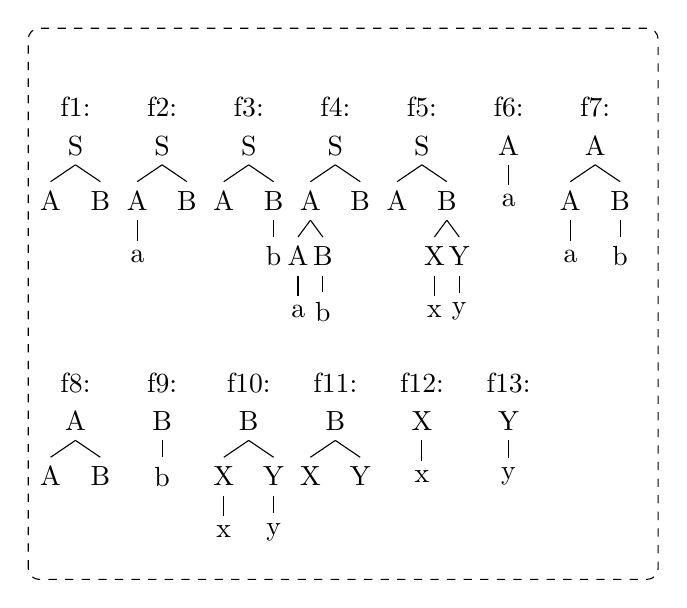
\begin{tikzpicture}
[node distance = 0 pt, sibling distance=18pt, level distance=20pt,level 2/.style={sibling distance=9pt},level 3/.style={sibling distance=9pt}]

\draw[black,dashed,join=round, inner frame sep=2cm and 2cm, rounded corners ] (0,3) rectangle (8,10);
%\node[fill = white, rectangle, draw] (treebank) at(3.5,10) {Fragments with non-zero weights};


\node (f1) at(0.6,9){f1:}
node [ below =of f1] {S}
child {node {A} 		}
child {node {B}		}
;


\node (f2) at(1.7,9){f2:}
node [ below =of f2] {S}
child {node {A} 	child {node {a}}
	}
child {node {B}	}
;

\node (f3)  at(2.8,9){f3:}
node [ below =of f3] {S}
child {node {A} 	}
child {node {B}	child{node {b}}
	}
;

\node (f4) at(3.9,9) {f4:}
node [ below =of f4] {S}
child {node {A} 	child{node {A}	child{node {a}}}
			child{node {B}	child{node {b}}}
	}
child {node {B}		}
;

\node (f5) at(5.0,9) {f5:}
node [ below =of f5] {S}
child {node {A} 		}
child {node {B}	child{node {X}	child{node {x}}}
			child{node {Y}	child{node {y}}}
	}
;

\node(f6) at(6.1,9) {f6:}
node [ below =of f6] {A}	
	child {node {a}}
;

\node(f7) at(7.2,9) {f7:}
node [ below =of f7]  {A} 	
	child{node {A}	child{node {a}}}
	child{node {B}	child{node {b}}}
;




\node(f8) at(0.6,5.5){f8:}
node [ below =of f8]  {A} 	
	child{node {A}	}
	child{node {B}	}
;

\node(f9) at(1.7,5.5) {f9:}
node [ below =of f9] {B}	
	child {node {b}}
;

\node(f10) at(2.8,5.5) {f10:}
node [ below =of f10]  {B} 	
	child{node {X}	child{node {x}}}
	child{node {Y}	child{node {y}}}
;

\node(f11) at(3.9,5.5) {f11:}
node [ below =of f11]  {B} 	
	child{node {X}	}
	child{node {Y}	}
;

\node(f12) at(5.0,5.5) {f12:}
node [ below =of f12] {X}	
	child {node {x}}
;

\node(f13) at(6.1,5.5) {f13:}
node [ below =of f13] {Y}	
	child {node {y}}
;
\end{tikzpicture}

\caption{All extracted fragments}
\label{f:fragments}
\end{figure}


Fragments can be combined in a \emph{derivation} to build syntactic structures. A step in a derivation is a composition, denoted by the symbol $\circ$. We follow the convention to only allow left-most derivations. This means that the left-most non-terminal node in a fragment $f_1$ must correspond to the root node of $f_2$ in order to derive $f_3=f_1\circ f_2$

For each fragment, the probability is estimated by counting how often it occurs in the treebank, compared to others with the same root. The probability of a derivation is the product of the probability of the fragments. Note that a single tree can be the result of different derivations. Therefore probability of a tree is the sum of the probabilities of all its derivations.

\subsection{Theoretical issues}
It has been argued that DOP (in its original formulation) is biased and inconsistent \cite{johnson2002}, both assumed to be bad properties of an estimator in general. As we will see, bias is not necessarily a bad thing. In fact, Zollman proves in  \cite{zollmann2005} that any non-overfitting estimator is biased. Furthermore, he shows that it is possible to define a DOP-estimator that is consistent.


\subsection{Practical issues}
In its original formulation, DOP takes the trees apart in all possible ways. The number of fragments is exponential in the length of the sentences, thus the size of the symbolic grammar would be far too huge to be computationally feasible. 
Different approaches have been taken to reduce the symbolic grammar, e.g. by sampling or by applying a smart algorithm. This appears to be far from trivial.


\subsection{Outlook}
Section~\ref{sec:Statistics} elaborates the notions of consistency and bias and their relation to overfitting.
In section~\ref{sec:Existing}, we outline two approaches that tackle the reduction of the symbolic grammars: \ddop{} and \dops{}. This report focuses on a comparison of these approaches. Theoretically, they differ in that \dops{}, unlike \ddop{}, has been proven to be consistent \cite{zollmann2005}. We investigate the differences between the grammars produced by \ddop{} \dops{}. The algorithms can be decomposed into two parts. We also analyze the impact of the partial choices by mutually using these parts.

Section~\ref{sec:Comparison} offers a detailed comparison of the two methods as well as a description of the experiments we conduct. In section~\ref{sec:Results}, we present our findings and provide an analysis. 



\section{Statistics: Bias and Consistency}\label{sec:Statistics}



% Distribution, sampling, estimation, corpus.
In contrast to \emph{competence} models that are the subject of most linguistic study, a \emph{performance} model of language is an estimate of the probability of observing a parse tree. It treats language as a statistical distribution over syntactic structures.

$$\Omega = $$

Using parse tree samples from the language, an estimator builds a statistical model. A parser then uses that statistical model to predict the correct parse tree of sentences.
A collection of parse tree samples is called a \emph{corpus} or \emph{treebank}.

$$  $$

% Expectation given a distribution, Loss, risk, mean squared difference, error.
In theory, an estimator should make exactly the right estimations of probabilities if it's given an infinite amount of data. That is to say, it should \emph{converge} to the true distribution. If an estimator converges in the limit, that estimator is \emph{consistent}.
However, given a finite amount of data, the estimator will probably not generate the correct probabilities. The distance between the true distribution and an estimate is called the \emph{loss} of that estimate. The loss can be defined in different ways, but the most popular is the \emph{mean squared difference}:

$$ \mathcal{L} $$

From a true distribution, it's possible to calculate the expected loss of an estimator trained on a treebank of a certain size. This is the \emph{risk} of that estimator given a sample size and a distribution.

$$ \mathcal{E} $$

%Other estimators:

%\emph{relative frequency}

%EWE, MLE



%- Why DOP*?



%- How do we prevent overfitting?

Bias is good.


\section{Existing Frameworks: Double-DOP and DOP$^*$}
%A description and comparison of Double-DOP and DOP*

A PTSG consists of the symbolic grammmar, i.e. a set of fragments, and the corresponding weights. In the general case of DOP, all fragments are extracted from all the trees in the treebank. The number of fragments is exponential in the length of the sentences, thus the total number of fragments extracted would be far too large for efficient computation. 
%DOP1: sample
Later models have therefore restricted the set of fragments in the grammar, thus improving computational efficiency. However, determining a proper subset of fragments to use is not trivial and this choice may negatively influence the performance of the grammar.

%Iets met Goodman? Die behoudt alleen kleine stukjes en speciale regels, maar daardoor geen expliciete representatie van 'productive units' (Sangati, einde van sectie 2)

In this section, we outline two approaches to constrain the extraction of fragments: \ddop and \dops. Furthermore, we discuss the similarities and dissimilarities for these two approaches. 

\subsection{\ddop}
In the following, we discuss \ddop{} as it was presented in \cite{sangati2011}. In this model, no unique fragments are extracted from the dataset: if a construction occurs in one tree only, it is probably not representative for the language. This is carried out by a dynamic algorithm using tree-kernels. It iterates over pairs of trees in the treebank, looking for fragments they have in common. In addition, only the largest shared fragment is stored. 

The symbolic grammar that is the output of this algorithmis not guaranteed to derive each tree in the training corpus. Therefore all one-level fragments, consitutuing the set of PCFG-productions, are also added.

After the extraction of the symbolic grammar, the weights are obtained. This is done in a second pass over the treebank, assessing the relative frequencies. 

The \ddop{} model has its main focus on determining the symbolic grammar. However, it was implemented with different estimators and maximizing objectives. Empirical results show that %

\paragraph{Consistency and bias}

\subsection{\dops}
In \dops{} \cite{zollmann2005}, a rather different approach is taken called held-out estimation. The treebank is split in two parts, the extraction corpus ($EC$) and a held-out corpus ($HC$). An initial set of fragments is extracted from the $EC$, containing all the fragments from its trees. The weights are then determined so as to to maximize the likelihood of $HC$, under the assumption that this is equivalent to maximizing the joint probability of the \emph{shortest derivations} of the trees in $HC$. All fragments that do not occur in such a derivation are removed from the symbolic grammar. Note that some trees in $HC$ may not be derivable at all. 

\paragraph{Consistency and bias}
\dops{} was claimed to be the first consistent (non-trivial) DOP-estimator, \cite{zollmann2005} provides a consistency proof. On the other hand \dops{} is  biased, but Zollmann shows how bias actually arises from generalization: no non-overfitting DOP estimator could be unbiased. Bias is therefore not prohibited but on the contrary a desirable property of an estimator.

In \cite{zuidema2006} it is argued that there is a problem with the consistency proof given for \dops{}, as well as the non-consistency proof for other DOP-estimators by \cite{johnson2002}. Zuidema points out that these proofs use a frequency-distribution test, whereas for DOP a weight-distribution test would be more appropriate. 
%Wat hiermee?

%
%\subsection{Comparison}
%Both \dops{} and \ddop{} restrict the symbolic grammar based on some notion of reoccurence of fragments. 
%
%In \ddop{} this is evident, it is explicit in the algorithm how (largest) reoccuring fragments are added to the grammar. From a computational point of view, this approach is very intuitive and can be implemented rather efficiently. However, the threshold (two) on the number of reoccurences might seem rather trivial. Indeed, \cite{sangati2011} reports experiments varying this threshold that show how performance drops for higher thresholds, with on the other hand a great reduction of the size of the grammar. A proper setting might well depend on the size and nature of the treebank used, and the computational costs one is willing to pay. In short, \ddop{} is computationally attractive but its theoretical foundation is not convincing us.
%%wel performance maar competence raadsel
%
%Theoretically,\dops{} is more appealing: we decide on the symbolic grammar by assessing which fragments are actually used in derivations. The main assumption is that shortest derivations are preferred. The splitting of the treebank makes this possible (otherwise the grammar would be terribly overfitted).
%
%
%
%\subsection{Preview}
%\dops{} is proven to be consistent and theoretically appealing. The computational problem of \dops{} is that, at first, the entire set of possible fragments is extracted from $EC$ and this set is reduced in a later phase. This comes with the need for huge storage and computation. In the next section, we investigate the possibility of reformulating the \dops{} approach with insights from the \ddop{} model to maintain the best of both worlds. 
%
%%\dops{} theoretically more appealing, \ddop{} computationally: lend properties of \ddop{} to implement \dops{}






\subsection{Comparison}
%The theoretical properties of \dops{} and \ddop{} differ:  
\dops{} and \ddop{} differ both in the set of fragments they extract and their estimation of the weights. To investigate the exact differences, we will view both steps separately.

Note that the \dops{} extraction needs another decision: in many cases, there are several shortest derivations possible. From now on, we add all fragments that occur in one of these shortest derivations to the symbolic grammar. Of course we need to adjust the weights (e.g. divide the frequency counts by the number of shortest derivations) so that no full tree gets a higher impact on the PTSG. We will keep to the original formulation of \dops{} in case no derivation is possible, i.e. not including any fragments for this tree.

\paragraph{Extraction}
\ddop{} uses tree kernels to find the maximal overlapping fragments of pairs of trees, which are added to the symbolic grammar. We will call this the \emph{maximal-overlap} method. \dops{} iteratively finds the shortest derivation of one tree given all the fragments of a set of trees, herafter the \emph{shortest-derivation} method. The example in figure \ref{f:differentSets} shows that the sets of extracted fragments from these methods does indeed differ.

\begin{figure}
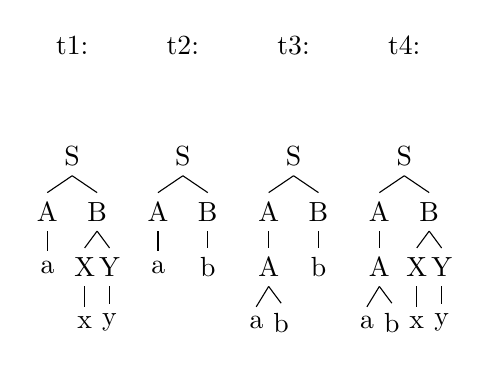
\begin{tikzpicture}
[node distance = 40 pt, sibling distance=18pt, level distance=20pt,level 2/.style={sibling distance=9pt},level 3/.style={sibling distance=9pt}]

\node (t1) {t1:}
node [ below of= t1] {S}
child {node {A} 	child {node {a}}
	}
child {node {B}	child{node {X}	child{node {x}}}
			child{node {Y}	child{node {y}}}
	}
;

\node [right of = t1] (t2) {t2:}
node [ below of= t2] {S}
child {node {A} 	child {node {a}}
	}
child {node {B}	child{node {b}}
	}
;

\node [right of = t2] (t3) {t3:}
node [ below of= t3] {S}
child {node {A} 	child {node {A}	child{node {a}}
						child{node {b}}
				}
	}
child {node {B}	child{node {b}}
	}
; 

\node [right of = t3] (t4) {t4:}
node [ below of= t4] {S}
child {node {A} 	child {node {A}	child{node {a}}
						child{node {b}}
				}
	}
child {node {B}	child{node {X}	child{node {x}}}
			child{node {Y}	child{node {y}}}
	}
;
\end{tikzpicture}
\caption{The fragment sets resulting from \emph{maximal-overlap} and \emph{shortest-derivation} extraction}
\label{f:differentSets}
\end{figure}

It is easy to see that the \dops{} extraction method does not depend on the corpus split: we can also try to find the shortest possble derivation using fragments from all the other trees. Likewise \ddop{} could be implemented using a split, comparing pairs that consist of a tree from each part of the corpus. Whether the corpus is split in two does only influence the size of the symbolic grammar and not its constitution.

Therefore, we will implement both extraction methods in a 1 vs the rest manner. In this way, we can analyse how the resulting symbolic grammars differ. The analysis will comprise the size of the resulting symbolic grammar and the relative number of fragments of certain depth. Furthermore, we might be able to find interesting patterns by manually looking at the fragments that were extracted by one of the systems only.s

\paragraph{Estimation}
The next step would be to compare the estimation methods: use either a split or the whole set of trees for both estimators. \ddop{} counts the occurences of fragments in the symbolic grammar, whereas \dops{} counts the occurrences in shortest derivations. Therefore, the extraction and estimation are best done simultaneously in the latter case. This comparison would involve a performance measure, such as the F1-score for correctly predicted parses.






























\section{Comparison} \label{sec:Comparison}
%The theoretical properties of \dops{} and \ddop{} differ:  
\dops{} and \ddop{} differ both in the set of fragments they extract and their estimation of the weights. To investigate the exact differences, we will view both steps separately.

\paragraph{Extraction}
\ddop{} uses a tree kernel approach to find the maximal overlapping fragments of pairs of trees, which are added to the symbolic grammar. We will call this the \emph{maximal-overlap} method. \dops{} iteratively finds the shortest derivation of one tree given all the fragments of a set of trees, hereafter the \emph{shortest-derivation} method. 

It is easy to see that the \emph{shortest-derivation} extraction in itself does not depend on the corpus split: we can also find the shortest possible derivation using fragments from all the other trees. Likewise \ddop{} could be implemented using a split, comparing all trees in the $HC$ to all trees in the $EC$.
We will refer to these methods as \emph{full} and \emph{split} estimation.

\paragraph{Estimation}

Both approaches use the relative frequencies of the fragments for the weights:
\begin{align}p(f)=\frac{count(f)}{\sum_{f'\in F_{root}(f)} count(f')}\end{align} 
Where $F_{root}(f)$ denotes the fragments in the grammar that have the same root as $f$.
However, in the \ddop{} case these values refer to exact counts of the fragments in the treebank, whereas in \dops{} they refer to occurrence of fragments in shortest derivations.


\ddop{} determines the weights of the fragments in the symbolic grammar in a separate run over the treebank, to obtain exact counts. We use the relative frequency estimate to assign weights to the fragments. \dops{} on the other hand counts the occurrence in shortest derivations of the fragments, and normalizes relative to counts of fragments with the same root.

\paragraph{Smoothing}
To maximize coverage of the grammar, both \ddop{} and \dops{} add PCFG rules to the grammar. In \ddop{} this is done before the estimation, such that the CFG rules are treated as if they were extracted as maximal overlapping fragments. \dops{} is smoothed by calculating the weight of the unparsed sentences: $p_{unkn}$, and distributes this probability mass over the PCFG grammar.




\paragraph{Example}
\FloatBarrier
This example clarifies how the grammars that result from \ddop{} and \dops{} can actually differ. Recall our toy treebank from figure \ref{f:treebank} and the fragments in figure \ref{f:fragments}. 
Applying the maximal overlap extraction and shortest derivation extraction with full estimation to this treebank, yields the weights in table \ref{t:weights}.

Note the remarkable differences in the weight distributions. For example, $f_1$ gets a weight of $p_k\times 0.5$ in the maximal overlap approach, and zero in the shortest derivation case. Of course, the sparsity of the data contributes much to these extreme variations. However, the observed differences encourage us to investigate these two approaches into more depth.

%TODO: smoothing weghalen uit DOUBLE-DOP

\begin{table*}[t]
\center
\begin{tabular}{c|p{.30\textwidth}c|p{.2\textwidth}l c}
&Maximal overlap$^*$&weight&Shortest deriv.$^{**}$&\multicolumn{2}{c}{weight$^{***}$}\\\hline
f1&(t1,t3), (t2,t4)	&4/12		&- 		&				&$p_u\times$	1/1\\     %P
f2&(t1,t2)		&2/12		&1b, 2a 	&$p_k\times$	2/8	&\\	 
f3&(t2,t3)		&2/12		&2b, 3b 	&$p_k\times$	2/8	&\\
f4&(t3,t4)		&2/12		&3a, 4b 	&$p_k\times$	2/8	&\\
f5&(t1,t4)		&2/12		&1a, 4a 	&$p_k\times$	2/8	&\\
f6&(t1,t3), (t1,t4), 
(t2,t3), (t2,t4)	&4/6		&1a, 2b 	&$p_k\times$	2/4	+& $p_u\times$	1/2\\	%P
f7&- 			&0		&3b, 4a 	&$p_k\times$	2/4	&\\
f8&CFG rule		&2/6		&- 		&				&$p_u\times$	1/2\\	%P
f9&(t2,t3), (t2,t4), 
(t3,t4)		&4/6		&2a, 3a 	&$p_k\times$	2/4	+&$p_u\times$	1/2\\	%P
f10&- 			&0		&1b, 4b 	&$p_k\times$	2/4	&\\
f11&CFG rule	&2/6		&- 		&				&$p_u\times$1/2\\	%P
f12&CFG rule	&2/2		&- 		&				&$p_u\times$1/1\\	%P
f13&CFG rule	&2/2		&- 		&				&$p_u\times$1/1\\	%P
\end{tabular}

\caption{The weights assignment according to both extraction methods in a full estimation manner.\\
{\footnotesize$^*$ The fragment occurs in the maximal overlap of these pairs of trees\\
$^{**}$ For this dataset, two shortest derivations exist for each tree:
$t_1=f_5\circ f_6$~(1a)~or~$t_1=f_2\circ f_{10}$~(1b), 	$t_2=f_2\circ f_8$~(2a)~or~$t_2=f_3\circ f_6$~(2b),
$t_3=f_4\circ f_8$~(3a)~or~$t_3=f_3\circ f_7$~(3b),	$t_4=f_5\circ f_7$~(4a)~or~$t_4=f_4\circ f9$~(4b)\\
$^{***}$ Smoothing: $p_u$ is short for $p_{unkn}$, $p_k = 1- p_{unkn}$
}
}
\label{t:weights}
\end{table*}




\subsection{Experiments}
%Description of our implementation, how does it resemble Double-DOP and DOP*? What are the differences? What are the theoretical capabilities? 

We compare the original formulation of \ddop{} and \dops{}, i.e. maximal overlap with full estimation and shortest derivation with split estimation. Furthermore, we add a new estimator that is a hybrid of the two: maximal overlap with split estimation. We have not been able to provide an efficient  implementation of shortest derivation extraction with full estimation.


Estimation and parsing were done with the {\tt disco-dop} framework \footnote{http://staff.science.uva.nl/~acranenb/discodop/}.


\paragraph{Data}
We use the \emph{Wall Street Journal}~(WSJ) section of the Penn Treebank for our experiments. \dops{} has only been applied to the Dutch OVIS corpus in \cite{zollmann2005}, which contains relatively small and (therefore) easy sentences. Therefore we are curious about its performance on the WSJ.

The corpus was preprocessed in {\tt disco-dop} by removing functions and binarizing the trees by Markovization (h=1, v=1). %\footcite{klein2003}. 

\paragraph{Algorithm}
First, we find the maximally overlapping fragments of all trees in the corpus, which corresponds to \ddop, and we call the \emph{Full Maximum Overlap} approach.
Then, we randomly split the corpus ten times in two equally-sized parts, called $EC$ and $HC$. For each split, build a DOP-reduction grammar from $EC$ and use it to find the shortest derivations (\emph{Split Shortest Derivations}) of the trees in $HC$, which corresponds to \dops{}. Additionally, we find the maximally overlapping fragments and estimate their weights from the $EC$. We'll call this \emph{Split Maximum Overlap}.

The results for the different splits were interpolated and the resulting grammars were smoothed as described above. For finding $p_{Unkn}$, the weight of unparsable sentences in the \dops{} estimation, we needed to find the trees that had not been derived in any split. This was done by comparing each set of underived trees with the $HC$ sets of every split.

\paragraph{Parsing}
The input for the parser consisted of sentences with a POS-tag attached to each word. The parser matches fragments to the whole pair (word and POS-tag) when the word is known, but only uses the POS tag in case the word is unknown.


% Estimating all grammars took 45 hours on 16 CPU cores.

% \paragraph{Questions}
% Comparing \dops{} and \ddop{}: Which estimator gives more weight to large fragments? Is this related to consistency?

% Comparing \ddop{} and Split Double-DOP: What influence does a split have on performance and size of a grammar? How do the fragment weight distributions differ?

% Comparing Split Double-DOP and \dops{}: Assuming that a larger weight in \dops{} corresponds to `usefulness' in parsing, what determines whether a fragment is useful?



\section{Results}\label{sec:Results}
%Empirical results of our implementation (on the WSJ corpus?)

\begin{figure}
\center
\includegraphics[width=\linewidth]{../data/plots/plot0.png}
\end{figure}


\begin{figure}
\center
\includegraphics[width=\linewidth]{../data/plots/plot1.png}
\end{figure}


\begin{figure}
\center
\includegraphics[width=\linewidth]{../data/plots/plot2.png}
\end{figure}


\begin{figure}
\center
\includegraphics[width=\linewidth]{../data/plots/plot3.png}
\end{figure}
\section{Conclusion}
%Discussion, future work

%Split (held-out est) reduces bias towards large fragments


%Double-DOP: best performance

%Performance not correlated with consistency of the method

%Shortest derivation, very short grammar. But not as useful as it would seem: bad performance

\paragraph{Future work}
% analysis of other DOP grammars, 
%more elaborate analysis: possibly clustering on features such as depth, number of substitution sites and terminals

% is consistency indeed a valuable property at all?





%\bibliographystyle{ieeetr}
%\bibliography{bibliography}

\bibliographystyle{acl2014}
\bibliography{bibliography}

\end{document}
